\documentclass[a4paper, 12pt]{article}
\usepackage [MeX]{polski}
\usepackage [utf8] {inputenc}
\usepackage {hyperref}
\usepackage{graphicx}
\usepackage[nottoc,numbib]{tocbibind}
\usepackage{algpseudocode}
\title {Projekt z przedmiotu GIS - sprawozdanie II}
\author{Marek Jasiński, Przemysław Piotrowski}

\begin{document}

\maketitle

\section{Treść zadania}

\paragraph{Temat zadania}
Znajdowanie zbioru najkrótszych ścieżek pomiędzy parą wybranych lub wylosowanych wierzchołków grafu przy awaryjnych krawędziach.

\paragraph{Opis zadania}
Muszą być spełnione następujące warunki: a)pierwsza wygenerowana ścieżka: najkrótsza ścieżka pomiędzy wybraną parą wierzchołków b)każda następna wygenerowana ścieżka posiada krawędź różną od co najmniej jednej krawędzi ścieżki z punktu a) i minimalną długość. Krok b) jest powtarzany kolejno aż do wyczerpania wszystkich krawędzi ścieżki z punktu a) Dane do projektu: G=(V,E) - graf o zadanej strukturze, wylosowana lub wybrana para wierzchołków. Zastosowanie: wyznaczanie ścieżek rezerwowych w sieci w sytuacji awarii pojedynczej krawędzi sieci. Literatura: N.Christofides, Graph Theory - an algorithmic approach, Academic Press 1975, str. 150- 157, 167-170. M.Sysło, N.Deo, J.Kowalik, Algorytmy optymalizacji dyskretnej, PWN 1995. N.Deo, Teoria grafów i jej zastosowania w technice i informatyce. PWN 1980.

\section{Algorytmy}

\subsection{Wyszukiwanie alternatywnych ścieżek}
\label{wyszukiwanie}
Graf jest wewnętrznie reprezentowany w~postaci listy sąsiedztwa, której implementację dostarcza biblioteka Boost Graph \cite{bgl}. Pomimo, że biblioteka dostarcza implementację algorytmu znajdującego najkrótszą ścieżkę pomiędzy dwoma wierzchołkami, zaimplementowaliśmy własny algorytm oparty na algorytmie Dijkstry. Ogólny algorytm polega na znalezieniu najkrótszej ścieżki pomiędzy wierzchołkami źródłowym i~docelowym oraz wykorzystaniu jej do dalszego przetwarzania. Kolejne krawędzie z~tej ścieżki są tymczasowo usuwane, aby uruchamiać algorytm znajdywania najkrótszej ścieżki, który dostarcza alternatywną ścieżkę dla awaryjnej krawędzi. Warto zwrócić uwagę na to, że mogą istnieć krawędzie, których usunięcie spowoduje, że graf przestanie być spójny. Takie krawędzie oznaczane są kolorem czerwonym, jako krytyczne. Nie ma alternatywnych ścieżek w~grafie dla krawędzi krytycznych.

Złożoność algorytmu Dijkstry zależy od liczby wierzchołków $V$ i krawędzi $E$. O rzędzie tej wielkości decyduje sposób implementacji kolejki priorytetowej wykorzystywanej do pobierania wierzchołka o najmniejszym dystansie. W przypadku naiwnej implementacji poprzez tablice złożoność ta wynosi $O(V^2)$. W naszym programie zastosowaliśmy implementację kolejki opartą na stercie. W tym przypadku złożoność wynosi $O(E \log V)$. Wariant ten jest znacznie lepszy dla grafów rzadkich, którymi są sieci małego świata.

Rozpatrywany problem ma złożoność $O(P_{avg}*O_{Dijkstra})$, gdzie $P_{avg}$ to średnia długość ścieżki w grafie, natomiast $O_{Dijkstra}$ to złożoność algorytmu Dijkstry. Wynika to z podejścia widocznego w poniższym pseudokodzie.
\begin{algorithmic}
\State $\mathbf{Extern}\ graph\ \mathit{\# struktura\ grafu}$
\State $\mathbf{Extern}\ s, t\ \mathit{\# wierzchołki\ startowy\ i\ końcowy}$
\State
\State $emergencyPaths \gets [\ ]$
 \State $path \gets shortestPath(s, t, graph)$
\For{$edge\ e\ \mathbf{in}\ path$}
\State $graph.removeEdge(e)$
\State $emergencyPath \gets shortestPath(s, t, graph)$
\State $emergencyPaths.append(\ pair(e, emergencyPath)\ )$
\State $graph.addEdge(e)$
\EndFor
\State \Return{$path, emergencyPaths$}
\end{algorithmic}
Jak widać pętla wykonuje się średnio tyle razy, ile wynosi średnia długość ścieżki w grafie. W pętli najbardziej czasochłonną procedurą jest znalezienie najkrótszej ścieżki (funkcja $shortestPath$). Jej złożoność zależy od złożoności obliczeniowej algorytmu Dijkstry oraz odczytania ścieżki od $t$ do $s$, czyli wynosi $f = O_{Dijkstra}+ P_{avg}$. Drugi człon ma jednak wolniejszy stopień wzrostu, w związku z czym można przyjąć $O_{shortestPath}=O(f)=O(O_{Dijkstra}+ P_{avg}) = O(O_{Dijkstra}) = O(E \log V)$.
W związku z powyższym złożoność algorytmu to $O_{alg} = O( P_{avg}E \log V)$.

\subsection{Generowanie grafów}
\label{generowanie}
Wygenerowane grafy odwzorowują sieci małego świata\cite{amaral2000classes}. Oznacza to, że większość wierzchołków nie sąsiaduje ze sobą, ale pomiędzy większością par wierzchołków można znaleźć ścieżkę składającą się z małej liczby krawędzi. Sieci takie często obserwowane są np. w sieciach społecznościowych. Krawędź oznacza wtedy, że dwie osoby się znają.

Tworzenie przykładowego grafu małego świata składa się z dwóch kroków. Pierwszym z nich jest stworzenie grafu o regularnej strukturze. Przykład zaprezentowany jest na Rys. \ref{fig:regul}. Następnie należy dla każdej z krawędzi wylosować, czy powinna ona zostać przepięta, czy też nienaruszona. W efekcie powstaje graf jak na Rys. \ref{fig:pomiesz}. Dla większej liczby wierzchołków graf widocznie nabiera cech ,,małego świata''. Widoczne jest to na Rys. \ref{fig:bignetwork}.

\begin{figure}[ht]
\begin{minipage}[b]{0.45\linewidth}
\centering
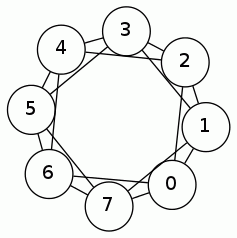
\includegraphics[width=\textwidth]{regularny.png}
\caption{\em Graf o regularnej strukturze}
\label{fig:regul}
\end{minipage}
\hspace{0.5cm}
\begin{minipage}[b]{0.45\linewidth}
\centering
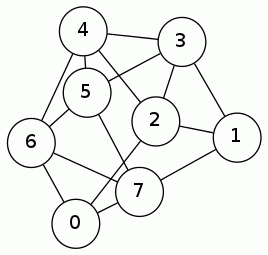
\includegraphics[width=\textwidth]{pomieszany.png}
\caption{\em Graf po przemieszaniu krawędzi}
\label{fig:pomiesz}
\end{minipage}
\end{figure}

\begin{figure}[!htbp]
\centering
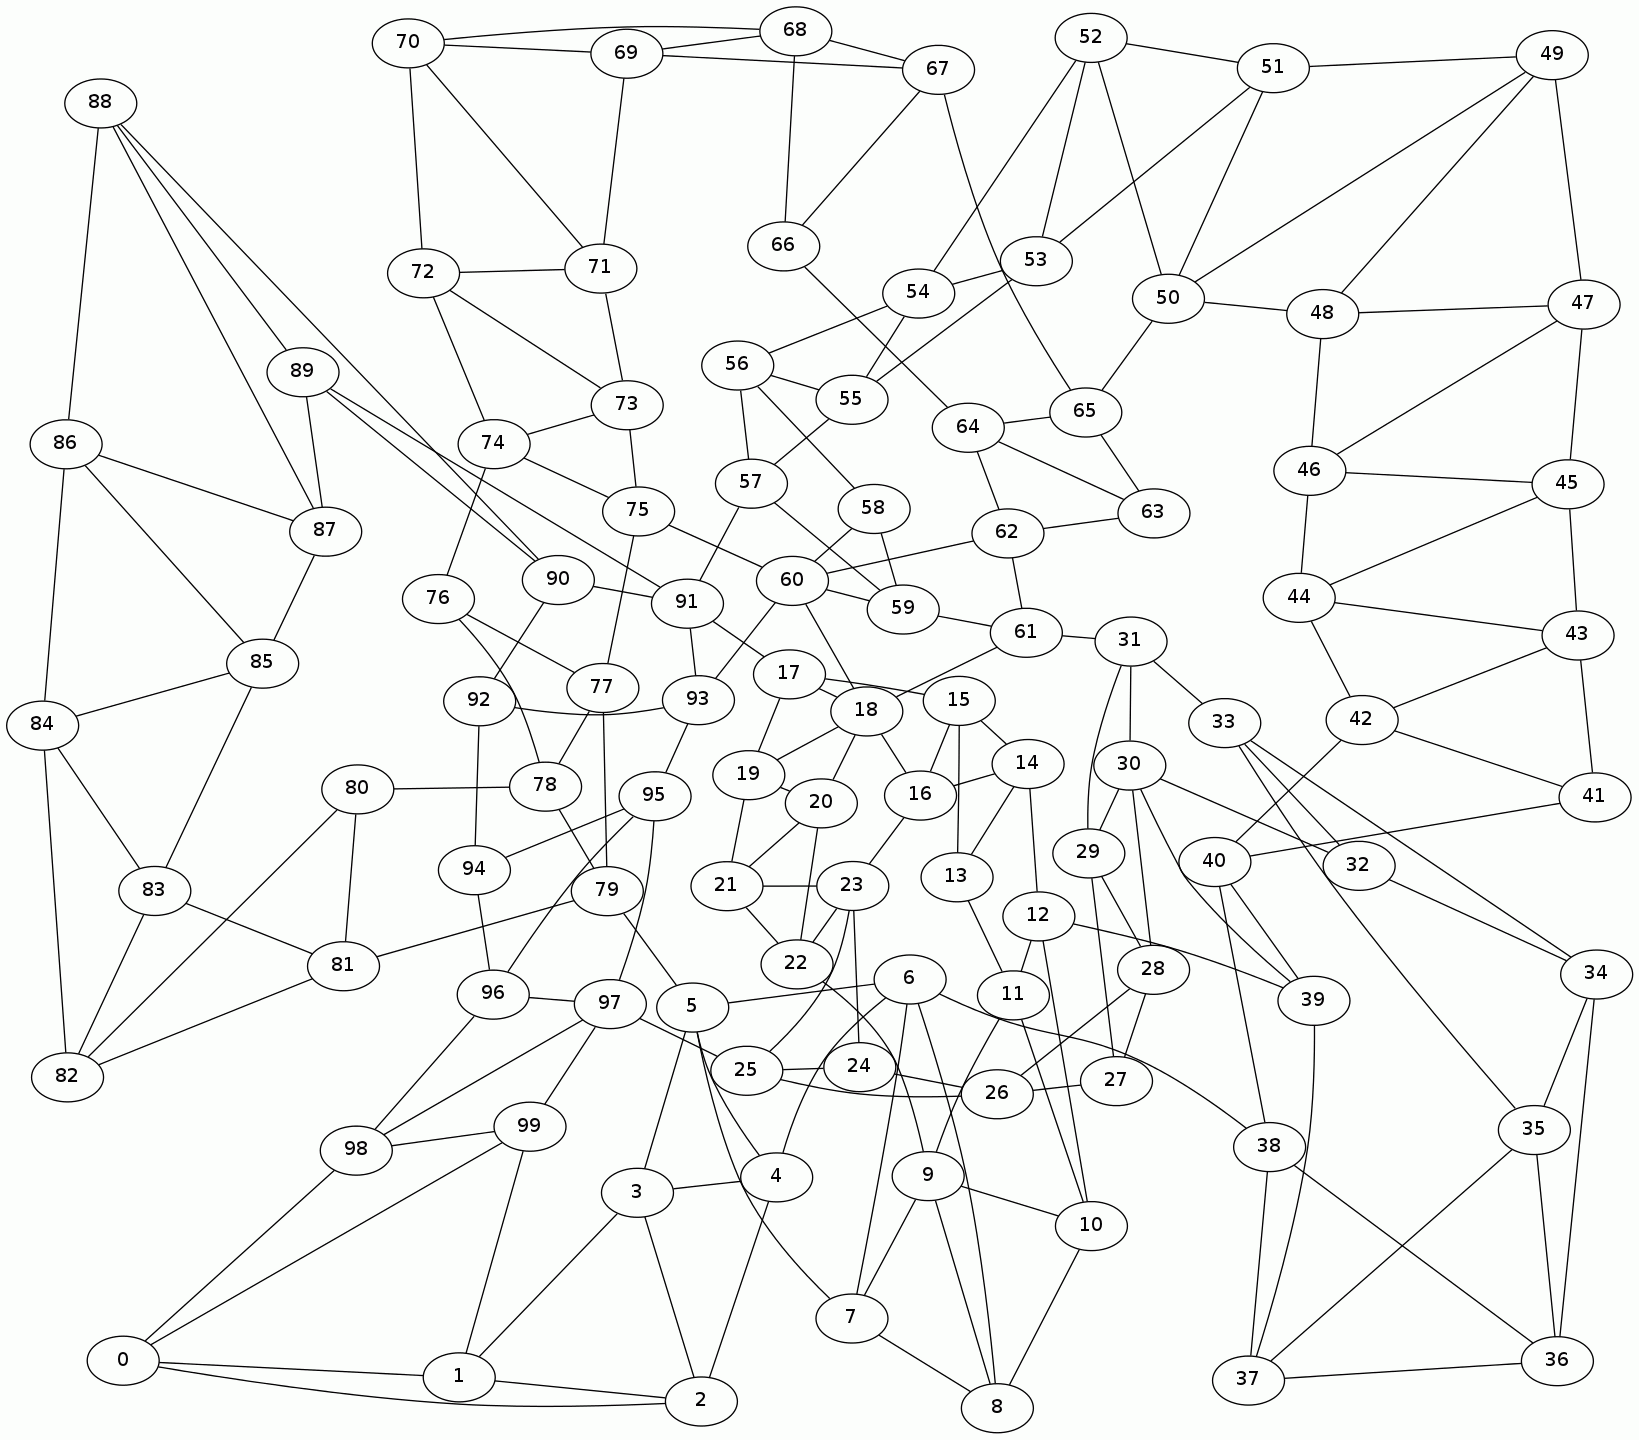
\includegraphics[scale=0.23]{biggraph.png}
\caption{\em Duży graf wygenerowany przez generator. Posiada cechy małego świata.}
\label{fig:bignetwork}
\end{figure}

\section{Programy}

Na potrzeby projektu zrealizowaliśmy dwa programy. Pierwszy z nich to właściwy program realizujący algorytm wyszukiwania najkrótszej ścieżki w grafie oraz ścieżek alternatywnych. Drugi jest generatorem grafów mających cechy ,,małego świata''. Nazwaliśmy je odpowiednio {\it ap} od {\it Alternate Path} oraz {\it gg} od {\it Graph Generator}. Obydwa programy zostały napisane w języku C++ i wykorzystują bibliotekę Boost Graph \cite{bgl} do wewnętrznej reprezentacji grafu w postaci listy sąsiedztwa. Oprogramowanie tworzyliśmy i uruchamialiśmy na dwóch platformach: Linux oraz Mac OS X. W skład projektu wchodzi plik {\it Makefile} służący do budowy projektu. Po wydaniu polecenia {\it make} w głównym katalogu projektu następuje kompilacja plików źródłowych, której rezultatem są pliki wykonywalne {\it ap} oraz {\it gg}.

\subsection{Właściwy program}

Program przyjmuje na wejściu graf oraz dwa wierzchołki: źródłowy i~docelowy. Graf musi być grafem nieskierowanym z~ważonymi krawędziami (wagi nieujemne) bez krawędzi równoległych. Graf jest zadawany w~pliku tekstowym. Format tego pliku jest zgodny z~formatem DOT \cite{dot}. Parametrami programu są:

\begin{itemize}
\item nazwa pliku tekstowego zawierającego opis grafu w~formacie DOT,
\item nazwa wierzchołka źródłowego (ang. {\it source}) i~nazwa wierzchołka docelowego (ang. {\it target}),
\item nazwa katalogu na pliki wynikowe.
\end{itemize}

Przykładowe wywołanie programu może wyglądać w~ten sposób:

\begin{verbatim}
$ ./ap graph.dot -s w1 -t w5 -o output
\end{verbatim}

Na skutek takiego wywołania program odczytuje graf z pliku {\it graph.dot}, znajduje najkrótszą ścieżkę pomiędzy wierzchołkami {\it w1} i {\it w5} oraz alternatywne ścieżki, a pliki będące wynikiem działania zapisuje w katalogu {\it output}. Program wspiera również dodatkowe opcje, które były użyteczne podczas testów i eksperymentów:

\begin{itemize}
\item \texttt{--no-report} -- powoduje, że nie jest generowany plik raportu, o którym mowa dalej,
\item \texttt{--no-html} -- powoduje, że nie są generowane pliki HTML wizualizujące rezultat działania programu.
\end{itemize}

Dostępne opcje programu wraz z krótkim opisem można przejrzeć po uruchomieniu programu z parametrem \texttt{--help}:

\begin{verbatim}
$ ./ap --help
Usage: ap [options]
Options::
  -h [ --help ]         Produce help message
  -f [ --file ] arg     Input graph filename (obligatory)
  -s [ --source ] arg   Source vertex name (obligatory)
  -t [ --target ] arg   Target vertex name (obligatory)
  -o [ --outdir ] arg   Output directory name (obligatory)
  --no-report           If specified, report won't be generated
  --no-html             If specified, HTML won't be generated
\end{verbatim}

Przykładowy plik z~zadanym grafem wejściowym w formacie DOT może wyglądać~w ten sposób:

\begin{verbatim}
/* graph.dot */
graph G {
	w1 -- w2 [weight=1];
	w2 -- w3 [weight=1];
	w1 -- w4 [weight=1];
	w4 -- w2 [weight=1];
	w2 -- w5 [weight=1];
	w5 -- w3 [weight=1];
}
\end{verbatim}

Plik opisujący graf może być przygotowany ręcznie, zostać pobrany z~Internetu, a~także może być wygenerowany przy pomocy naszego drugiego programu, tj. generatora grafów.

Wizualizację rezultatu działania programu zapewnia program NEATO z~pakietu Graphviz \cite{gv}. Służy on do rysowania grafów nieskierowanych. Program NEATO jest wywoływany z poziomu naszego programu. Za pomocą programu NEATO generowane są pliki, na podstawie których nasz program generuje strony HTML. Na stronach można zobaczyć, jak wyglądają najkrótsza ścieżka pomiędzy wierzchołkami źródłowym i~docelowym oraz najkrótsze ścieżki alternatywne (po kliknięciu na krawędź, którą uznaje się za awaryjną). Przykładowa zawartość stron może wyglądać jak na Rys. \ref{fig:picture1} i \ref{fig:picture2}.

\begin{figure}[ht]
\begin{minipage}[b]{0.45\linewidth}
\centering
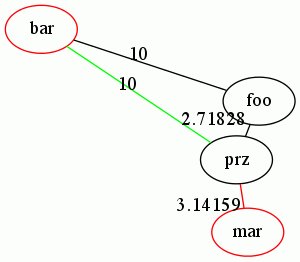
\includegraphics[width=\textwidth]{picture1.png}
\caption{\em Główny obrazek (na stronie index.html)}
\label{fig:picture1}
\end{minipage}
\hspace{0.5cm}
\begin{minipage}[b]{0.45\linewidth}
\centering
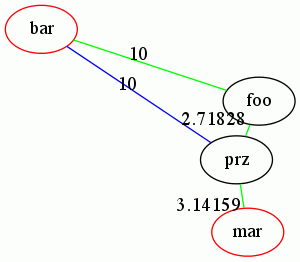
\includegraphics[width=\textwidth]{picture2.png}
\caption{\em Po kliknięciu na zieloną krawędź na głównym obrazku}
\label{fig:picture2}
\end{minipage}
\end{figure}

Na Rys. \ref{fig:picture1} widzimy najkrótszą ścieżkę pomiędzy wierzchołkami \texttt{mar} a \texttt{bar}. Została ona oznaczona na kolorowo. Składa się z~dwóch krawędzi. Na wypadek awarii krawędzi zielonej istnieje ścieżka alternatywna, która jest przedstawiona na Rys. \ref{fig:picture2}. Czerwona krawędź jest krytyczna - nie ma dla niej alternatywnych ścieżek. Usunięcie tej krawędzi spowodowałoby, że nie byłoby ścieżki pomiędzy wierzchołkami \texttt{mar} a \texttt{bar}.

Drugim rezultatem działania programu jest plik \texttt{report.txt} zawierający informacje o~najkrótszej ścieżce oraz ścieżkach alternatywnych. Przy każdej ze ścieżek jest informacja o~koszcie (sumie wag krawędzi) i liczbie krawędzi (liczbie przeskoków). Plik raportu dla powyższego przykładu wygląda w~ten sposób:

\begin{verbatim}
Shortest path: mar--prz--bar Cost: 13.1416 Hops: 2
mar--prz | No emergency path
prz--bar | mar--prz--foo--bar Cost: 15.8599 Hops: 3
\end{verbatim}

\subsection{Generator grafów}

Danymi wyjściowymi generatora są grafy zapisane w formacie DOT. Parametrami generatora są:

\begin{itemize}
\item plik wyjściowy,
\item liczba wierzchołków,
\item liczba krawędzi prowadzonych z każdego z wierzchołków do następników,
\item prawdopodobieństwo przepięcia krawędzi.
\end{itemize}

Przykładowe wywołanie:

\begin{verbatim}
$ ./gg graph.dot -n 30 -e 2 -p 20
\end{verbatim}

Powoduje wygenerowanie do pliku {\it graph.dot} grafu o $30$ wierzchołkach, w którym z każdego wierzchołka prowadzone są dwie krawędzie do dwóch kolejnych wierzchołków, a krawędzie są losowo przepięte z prawdopodobieństwem $\frac{20}{100}$.

Dostępne opcje programu wraz z krótkim opisem można przejrzeć po uruchomieniu programu z parametrem \texttt{--help}:

\begin{verbatim}
$ ./gg --help
Usage: ./gg [options]
Options::
  -h [ --help ]         Produce help message
  -o [ --output ] arg   Result graph filename (obligatory)
  -n [ --num ] arg      Number of vertexes (obligatory)
  -e [ --edges ] arg    Number of edges (obligatory)
  -p [ --prob ] arg     Probability, that edge will be moved (obligatory)
\end{verbatim}

\section{Testy i eksperymenty}

Złożoność obliczeniowa programu została zbadana za pomocą skryptu, który korzysta z generatora grafów. Skrypt został napisany w języku Python, a jego nazwa to {\it analyze\_algorithm.py}. Na początku swojego działania generuje on graf używając parametrów grafu z pliku {\it config.py}. Następnie określoną liczbę razy losuje wierzchołki źródłowy i docelowy, aby uruchamiać właściwy program i mierzyć czas jego działania. Właściwy program uruchamiany jest z opcją \texttt{--no-html}, aby czas działania programu NEATO nie wpływał na ogólny czas działania właściwego programu. Skrypt zapisuje w plikach {\it *.csv}:

\begin{itemize}
\item czasy działania programu wraz z liczbą krawędzi ścieżki pomiędzy wylosowanymi wierzchołkami,
\item średnie czasy działania programu dla poszczególnych liczb krawędzi ścieżki.
\end{itemize}

Przykładowy wynik działania skryptu prezentuje Rys. \ref{fig:tabela1} i \ref{fig:tabela2}.

\begin{figure}[ht]
\begin{minipage}[b]{0.41\linewidth}
\centering
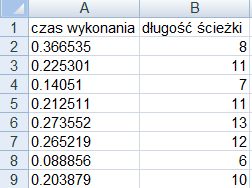
\includegraphics[width=\textwidth]{tabela1.png}
\caption{\em Czasy działania programu wraz z liczbą krawędzi ścieżki}
\label{fig:tabela1}
\end{minipage}
\hspace{0.5cm}
\begin{minipage}[b]{0.45\linewidth}
\centering
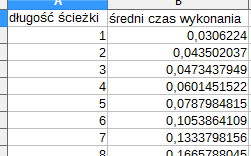
\includegraphics[width=\textwidth]{tabela2.png}
\caption{\em Średnie czasy działania programu dla poszczególnych liczb krawędzi w ścieżce}
\label{fig:tabela2}
\end{minipage}
\end{figure}

Na podstawie plików {\it *.csv} zostały wygenerowane wykresy z Rys. \ref{fig:wykres200V}, \ref{fig:wykres300V}, \ref{fig:wykres500V} i \ref{fig:wykres200V1000E}. Pokazują one zależność czasu działania programu od liczby krawędzi najkrótszej ścieżki pomiędzy dwoma wylosowanymi wierzchołkami. Jak widać, jest to zależność liniowa. Wynik eksperymentu potwierdza teoretyczne rozważania z rozdziału \ref{wyszukiwanie}.

\begin{figure}[!htb]
\centering
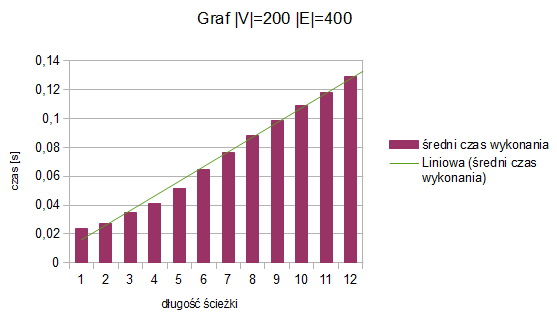
\includegraphics[scale=0.8]{tests/3/wykres.PNG}
\caption{\em Wykres średnich czasów działania programu dla poszczególnych liczb krawędzi w ścieżce}
\label{fig:wykres200V}
\end{figure}

\begin{figure}[!htb]
\centering
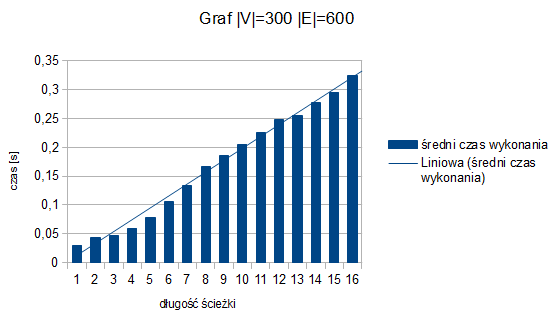
\includegraphics[scale=0.8]{tests/1/wykres.PNG}
\caption{\em Wykres średnich czasów działania programu dla poszczególnych liczb krawędzi w ścieżce}
\label{fig:wykres300V}
\end{figure}

\begin{figure}[!htb]
\centering
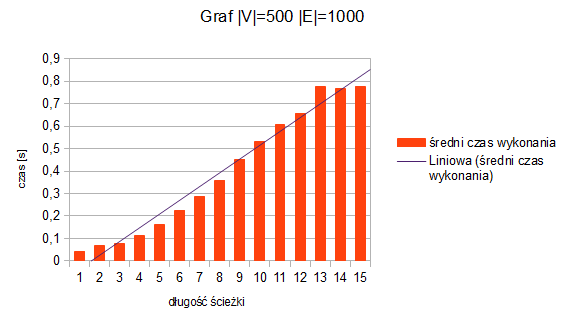
\includegraphics[scale=0.8]{tests/2/wykres.PNG}
\caption{\em Wykres średnich czasów działania programu dla poszczególnych liczb krawędzi w ścieżce}
\label{fig:wykres500V}
\end{figure}

\begin{figure}[!htb]
\centering
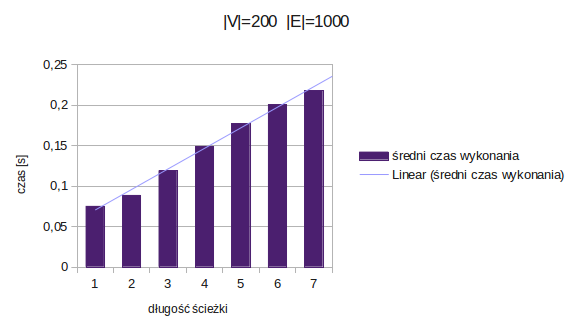
\includegraphics[scale=0.6]{tests/6/wykres.PNG}
\caption{\em Wykres średnich czasów działania programu dla poszczególnych liczb krawędzi w ścieżce}
\label{fig:wykres200V1000E}
\end{figure}

Wykres z Rys. \ref{fig:wykres-porownanie} porównuje zmierzone czasy dla dwóch grafów o tej samej liczbie krawędzi, wierzchołków i zbliżonych średnich liczbach krawędzi w ścieżce. Jak widać, czasy są do siebie zbliżone.

\begin{figure}[!htb]
\centering
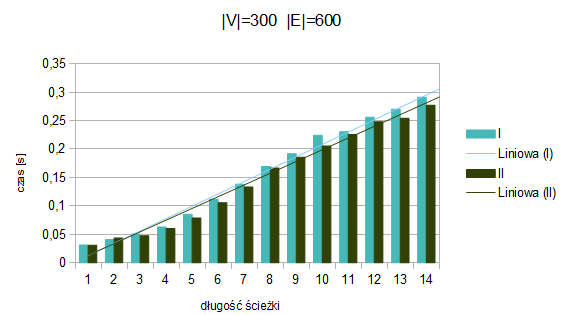
\includegraphics[scale=0.6]{tests/4/wykres.PNG}
\caption{\em Wykresy dla dwóch grafów o tej samej liczbie krawędzi i wierzchołków}
\label{fig:wykres-porownanie}
\end{figure}

\section{Podsumowanie}

Podsumowując, w ramach przedmiotu zostały napisane dwa programy oraz jeden skrypt do analizy algorytmu. Pierwszy program realizuje wymagania z opisu zadania projektowego. Tworzy on przyjazną reprezentację graficzną wyników. Drugi jest generatorem grafów ,,małych światów'' i pozwolił nam na wygenerowanie grafów niezbędnych do eksperymentów. Działanie aplikacji zostało przetestowane oraz została zbadana złożoność zastosowanego algorytmu opartego na algorytmie Dijkstry.

\begin{thebibliography}{}
\bibitem{dot} ,,The DOT Language'' \\ \url{http://www.graphviz.org/doc/info/lang.html}
\bibitem{bgl} ,,The Boost Graph Library'' \\ \url{http://www.boost.org/doc/libs/1_53_0/libs/graph/doc/index.html}
\bibitem{gv} ,,Graphviz - Graph Visualization Software'' \\ \url{http://www.graphviz.org/}
\bibitem{amaral2000classes} ,,Classes of small-world networks'', Amaral, Lu{\i}s A Nunes and Scala, Antonio and Barth{\'e}l{\'e}my, Marc and Stanley, H Eugene
\end{thebibliography}

\end{document}
